\documentclass{article} % Tạo một bản báo cáo

\usepackage[fontsize=13pt]{scrextend} % Chọn cỡ chữ 13 

\usepackage[T5]{fontenc}        % Sử dụng Tiếng Việt
\usepackage[utf8]{inputenc}     % Chuẩn utf8
\usepackage{url}
\usepackage[paperheight=29.7cm,paperwidth=21cm,right=2cm,left=3cm,top=2cm,bottom=2.5cm]{geometry}        % chuẩn A4, căn lề trái, phải, trên, dưới
%\usepackage[paperheight=29.7cm,paperwidth=21cm,right=2cm,left=3cm,top=2cm,bottom=2.5cm, twoside]{geometry} 
\usepackage{mathptmx}       % Time New Roman
\usepackage[hidelinks]{hyperref}
\usepackage{lipsum}
\usepackage{array}
\usepackage{graphicx} %Allows you to import images
\usepackage{float} %Allows for control of float positions
\usepackage{multirow} %Combine rows
\usepackage{titlesec}
\setcounter{secnumdepth}{4}
\titlespacing*{\section}{}{0pt}{30pt}
\titlespacing*{\subsection}{}{10pt}{0pt}
\titlespacing*{\subsubsection}{}{10pt}{0pt}
\titleformat*{\section}{\fontsize{16pt}{0pt}\selectfont \bfseries}
\titleformat*{\subsection}{\fontsize{14pt}{0pt}\selectfont \bfseries }
\titleformat*{\subsubsection}{\fontsize{13pt}{0pt}\selectfont \bfseries \itshape}
\titleformat*{\paragraph}{\fontsize{13pt}{0pt}\selectfont \itshape}
%\setlength{\parskip}{0.4cm}
%\linespread{1.2}
\usepackage{indentfirst}%  Thư viện thụt đầu dòng mỗi đoạn
\setlength{\parindent}{1cm} % Set khoảng cách thụt đầu dòng mỗi đoạn
\setlength{\parskip}{6pt} % Spacing after
\renewcommand{\baselinestretch}{1.2}% Giãn dòng 1.2

\usepackage[labelfont=bf]{caption}
% Thay đổi caption mặc định
\renewcommand{\figurename}{\fontsize{12pt}{0pt}\selectfont Hình}
\renewcommand{\tablename}{\fontsize{12pt}{0pt}\selectfont Bảng} 
\renewcommand{\contentsname}{\centering MỤC LỤC}
\renewcommand{\listfigurename}{\centering DANH MỤC HÌNH VẼ}
\renewcommand{\listtablename}{\centering DANH MỤC BẢNG BIỂU}
\renewcommand{\refname}{\centering TÀI LIỆU THAM KHẢO}
\renewcommand{\thefigure}{\thesection.\arabic{figure}}
\renewcommand{\thetable}{\thesection.\arabic{table}}
\renewcommand{\theequation}{\thesection.\arabic{equation}}

\captionsetup[figure]{labelsep=space}
\captionsetup[table]{labelsep=space}
\usepackage{ragged2e}
\usepackage{tikz}
\usetikzlibrary{calc}
% \setcounter{secnumdepth}{4}
%\usepackage{sectsty}
%\subsubsectionfont{\normalfont\itshape}
\usepackage{tabularx}
\newcolumntype{s}{>{\hsize=.4\hsize}X}
\newcolumntype{a}{>{\hsize=1.2\hsize}X}
\newcolumntype{d}{>{\hsize=0.25\hsize}X}
\usepackage{tocbasic}
\usepackage{enumitem}
\setlist{nosep}
\DeclareTOCStyleEntry[
  entrynumberformat=\entrynumberwithprefix{\figurename},
  dynnumwidth,
]{tocline}{figure}
\newcommand\entrynumberwithprefix[2]{#1\enspace#2}

\DeclareTOCStyleEntry[
  entrynumberformat=\entrynumberwithprefix{\tablename},
  dynnumwidth,
]{tocline}{table}
\newcommand\entrynumberwithprefix[2]{#1\enspace#2}

\usepackage{anyfontsize}
\newtheorem{theorem}{Định lý}[section]
\newtheorem{corollary}[theorem]{Hệ quả}
\newtheorem{lemma}[theorem]{Bổ đề}
\newtheorem{defn}[theorem]{Định nghĩa}

\begin{document}

\begin{titlepage}
\begin{tikzpicture}[overlay,remember picture]
\draw [line width=3pt]
    ($ (current page.north west) + (3.0cm,-2.0cm) $)
    rectangle
    ($ (current page.south east) + (-2.0cm,2.5cm) $);
\draw [line width=0.5pt]
    ($ (current page.north west) + (3.1cm,-2.1cm) $)
    rectangle
    ($ (current page.south east) + (-2.1cm,2.6cm) $); 
\end{tikzpicture}
\begin{center}
\vspace{-0.5cm}\fontsize{13pt}{0pt}\selectfont TRƯỜNG ĐẠI HỌC BÁCH KHOA HÀ NỘI \\
\textbf{\fontsize{16pt}{0pt}\selectfont VIỆN ĐIỆN TỬ - VIỄN THÔNG}
\vspace{0.5cm}
\begin{figure}[H]
	\centering
	
\includegraphics[height=2.26cm,width=1.53cm]{Images/logoBk.png}
\end{figure}
\vspace{1.5cm}
{\fontsize{24pt}{0pt}\selectfont ĐỒ ÁN}\\
\vspace{12pt}
\textbf{\fontsize{32pt}{0pt}\selectfont TỐT NGHIỆP ĐẠI HỌC}
\end{center}
\vspace{0.8cm}
\hspace{6pt}\textbf{\fontsize{14pt}{0pt}\selectfont Đề tài:}\\
\vspace{-20pt}
\begin{center}
    \textbf{\fontsize{20pt}{0pt}\selectfont NGHIÊN CỨU VÀ XÂY DỰNG THUẬT TOÁN}
    \textbf{\fontsize{20pt}{0pt}\selectfont ĐỊNH VỊ SỬ DỤNG CẢM BIẾN CẢM TÍNH}
    
\vspace{1.5cm}
\begin{tabular}{ l l }
\fontsize{14pt}{0pt}\selectfont Sinh viên thực hiện: & \fontsize{14pt}{0pt}\selectfont \vspace{6pt} NGUYỄN MAI CHI  \\ 
  & \fontsize{14pt}{0pt}\selectfont \vspace{6pt}Lớp ĐTVT 06 - K62 \\   
\fontsize{14pt}{0pt}\selectfont Giảng viên hướng dẫn: & \fontsize{14pt}{0pt}\selectfont TS. NGUYỄN TIẾN HÒA
\end{tabular}

\vspace{5.5cm}

\fontsize{14pt}{0pt}\selectfont Hà Nội, 5-2020    
\end{center}

\cleardoublepage
\thispagestyle{empty}
\begin{tikzpicture}[overlay,remember picture]
\draw [line width=3pt]
    ($ (current page.north west) + (3.0cm,-2.0cm) $)
    rectangle
    ($ (current page.south east) + (-2.0cm,2.5cm) $);
\draw [line width=0.5pt]
    ($ (current page.north west) + (3.1cm,-2.1cm) $)
    rectangle
    ($ (current page.south east) + (-2.1cm,2.6cm) $); 
\end{tikzpicture}
\begin{center}
\vspace{-0.5cm}\fontsize{13pt}{0pt}\selectfont TRƯỜNG ĐẠI HỌC BÁCH KHOA HÀ NỘI \\
\textbf{\fontsize{16pt}{0pt}\selectfont VIỆN ĐIỆN TỬ - VIỄN THÔNG}
\vspace{0.5cm}
\begin{figure}[H]
	\centering
	
\includegraphics[height=2.26cm,width=1.53cm]{Images/logoBk.png}
\end{figure}
\vspace{1.5cm}
\fontsize{24pt}{0pt}\selectfont ĐỒ ÁN\\
\vspace{12pt}
\textbf{\fontsize{32pt}{6pt}\selectfont TỐT NGHIỆP ĐẠI HỌC}
\end{center}
\vspace{0.8cm}
\hspace{6pt}\textbf{\fontsize{14pt}{0pt}\selectfont Đề tài:}\\
\vspace{-20pt}
\begin{center}
    \textbf{\fontsize{20pt}{0pt}\selectfont NGHIÊN CỨU VÀ XÂY DỰNG THUẬT TOÁN}
    \textbf{\fontsize{20pt}{6pt}\selectfont ĐỊNH VỊ SỬ DỤNG CẢM BIẾN CẢM TÍNH}
    
\vspace{1.5cm}
\begin{tabular}{ l l }
\fontsize{14pt}{0pt}\selectfont Sinh viên thực hiện: & \fontsize{14pt}{0pt}\selectfont  NGUYỄN MAI CHI \vspace{6pt} \\ 
  & \fontsize{14pt}{0pt}\selectfont Lớp ĐTVT 06 - K62 \vspace{6pt}\\   
\fontsize{14pt}{0pt}\selectfont  Giảng viên hướng dẫn:\vspace{6pt} & \fontsize{14pt}{0pt}\selectfont TS. NGUYỄN TIẾN HÒA\\
Cán bộ phản biện: &
\end{tabular}

\vspace{4.5cm}

\fontsize{14pt}{0pt}\selectfont Hà Nội, 5-2020    
\end{center}
\end{titlepage}
\cleardoublepage
\section*{\centering LỜI NÓI ĐẦU}
\thispagestyle{empty}
Phần này trình bày một cách rất khái quát (khoảng 1-2 trang) về bối cảnh hình thành và mục đích của đồ án. Lời cảm ơn đối với những tổ chức và cá nhân đã góp phần trong việc hoàn thiện đồ án (nếu có) nên đặt ở cuối mục này.
\cleardoublepage

\section*{\centering LỜI CAM ĐOAN}
\thispagestyle{empty}
Tôi là NGUYỄN MAI CHI, mã số sinh viên YYY, sinh viên lớp ZZZ, khóa TTT. Người hướng dẫn là TS. NGUYỄN TIẾN HÒA. Tôi xin cam đoan toàn bộ nội dung được trình bày trong đồ án Nghiên cứu và xây dựng thuật toán định vị sử dụng cảm biến quán tính là kết quả quá trình tìm hiểu và nghiên cứu của tôi. Các dữ liệu được nêu trong đồ án là hoàn toàn trung thực, phản ánh đúng kết quả đo đạc thực tế. Mọi thông tin trích dẫn đều tuân thủ các quy định về sở hữu trí tuệ; các tài liệu tham khảo được liệt kê rõ ràng. Tôi xin chịu hoàn toàn trách nhiệm với những nội dung được viết trong đồ án này.

\vspace{6pt}
\hspace{7cm}Hà Nội, ngày 28 tháng 11 năm 2020

\hspace{9cm}\textbf{Người cam đoan}

\vspace{2cm}
\hspace{8.65cm}\textbf{NGUYỄN MAI CHI}
\cleardoublepage

% This is the table of contents stuff
\addtocontents{toc}{\protect\thispagestyle{empty}}
\tableofcontents 
\thispagestyle{empty}
\cleardoublepage

\pagenumbering{roman}
\section*{\centering DANH MỤC KÝ HIỆU VÀ CHỮ VIẾT TẮT}
\phantomsection \addcontentsline{toc}{section}{\numberline{}DANH MỤC KÝ HIỆU VÀ CHỮ VIẾT TẮT }
\begin{table}[H]
\centering
\begin{tabularx}{0.8\textwidth} { 
  >{\Raggedleft\arraybackslash}X 
  >{\Raggedleft\arraybackslash}X[2]}
 
IFFT& Inverse Fast Fourier Transform\\

SNR & Signal-to-Noise Ratio  \\
BER & Bit Error Rate\\
SER & Symbol Error Rate \\
ISI & Inter Symbol Interference \\
\end{tabularx}
\end{table}
\cleardoublepage

%\list of figures
\listoffigures
\phantomsection \addcontentsline{toc}{section}{\numberline{}DANH MỤC HÌNH VẼ }
%\addcontentsline{toc}{section}{\numberline{}DANH MỤC HÌNH VẼ \dotfill}
\cleardoublepage

%\list of tables
\listoftables
\phantomsection \addcontentsline{toc}{section}{\numberline{}DANH MỤC BẢNG BIỂU}
\cleardoublepage

% abstract
\section*{\centering TÓM TẮT}
\phantomsection \addcontentsline{toc}{section}{\numberline{}TÓM TẮT}
Phần này trình bày những mục đích và các kết luận quan trọng nhất của đồ án bằng cả hai thứ tiếng: tiếng Việt (khoảng 1 trang) rồi đến tiếng Anh (khoảng 1 trang).
%\end{flushleft}
\cleardoublepage

\pagenumbering{arabic}
\section*{\centering  CHƯƠNG 1. CHƯƠNG MỞ ĐẦU}
\setcounter{section}{1}
\phantomsection \addcontentsline{toc}{section}{\numberline{}CHƯƠNG 1.  CHƯƠNG MỞ ĐẦU}
Phần mở đầu giới thiệu vấn đề mà đồ án cần giải quyết, mô tả được các phương pháp hiện có để giải quyết vấn để, trình bày mục đích của đồ án song song với việc giới hạn phạm vi của vấn đề mà đồ án sẽ tâp trung giải quyết. Phần này cũng sẽ giới thiệu tóm tắt cấu trúc đồ án và nội dung tương ứng của các phần sẽ lần lượt được trình bày ở các chương tiếp theo.

Nội dung chính của một đồ án tốt nghiệp thường bao gồm:
\begin{itemize}[itemsep=6pt]
    \item Phần mở đầu giới thiệu về đề tài.
    \item Một chương giới thiệu về cơ sở lý thuyết.
    \item Một hoặc nhiều chương trình bày các vấn đề về tính toán và thiết kế.
    \item Một chương mô tả các thí nghiệm và kết quả thu được.
\end{itemize}
\cleardoublepage
% This is main body stuff
\section*{\centering  CHƯƠNG 2. CƠ SỞ LÝ THUYẾT}
\setcounter{section}{2}
\setcounter{subsection}{0}
\setcounter{figure}{0}
\setcounter{table}{0}
\phantomsection \addcontentsline{toc}{section}{\numberline{}CHƯƠNG 2.  CƠ SỞ LÝ THUYẾT}
Mỗi chương sẽ bắt đầu bằng một đoạn giới thiệu các phần chính được trình bày trong chương đó, dài khoảng từ 5 đến 10 dòng và kết thúc bằng một đoạn tóm tắt các kết luận chính của chương. Chú ý phân bố chiều dài mỗi chương cho cân đối và hợp lý.
\subsection{Một số lưu ý khi trình bày đồ án}
Sau đây là một số lưu ý quan trọng các bạn cần nhớ nhé:
\subsubsection{Nộp đồ án}
Sinh viên (hoặc nhóm sinh viên với tối đa 3 thành viên làm chung một đề tài) nộp 02 quyển đồ án tốt nghiệp tại văn phòng bộ môn của giảng viên hướng dẫn trước ngày bảo vệ ít nhất một tuần. Một quyển đồ án cần có các đặc điểm sau:
\begin{itemize}[itemsep=6pt]
    \item Được \textbf{in hai mặt} nhằm tiết kiệm không gian lưu trữ.
    \item Đóng bìa mềm, bên ngoài là lớp bóng kính.
    \item Số trang: 50-150 trang, không kể phần phụ lục.
    \item Phải có chữ ký của sinh viên sau Lời cam đoan và của giảng viên hướng dẫn.
\end{itemize}
\subsubsection{Phụ lục}
Phụ lục (nếu có) chứa các thông tin quan trọng có liên quan đến đồ án nhưng nếu để trong phần chính sẽ gây rườm rà. Thông thường các chi tiết sau thường được để trong phần phụ lục: kết quả thô (chưa qua xử lý), mã nguồn phần mềm, thông số kỹ thuật chi tiết của linh kiện, hình ảnh minh họa thêm, v.v.
\subsubsection{Tài liệu tham khảo}
\paragraph{Cách liệt kê}\mbox{}

Áp dụng cách liệt kê theo quy định của IEEE. Theo đó, tài liệu tham khảo được đánh số thứ tự trong ngoặc vuông, ví dụ \cite{jakobsson2020physical}, \cite{byrne2014effect}. Thứ tự liệt kê là thứ tự xuất hiện của tài liệu được trích dẫn trong đồ án. Tài liệu tham khảo đã liệt kê bắt buộc phải được trích dẫn trong phần nội dung của đồ án. Tài liệu tham khảo cần có nguồn gốc rõ ràng và phải từ nguồn đáng tin cậy. Hạn chế trích dẫn tài liệu tham khảo từ các website, từ Wikipedia.\vspace{-12pt}
\paragraph{Các loại tài liệu tham khảo}\mbox{}

Các nguồn tài liệu tham khảo chính là sách, bài báo trong các tạp chí, bài báo trong các hội nghị khoa học, và các tài liệu tham khảo khác trên Internet.

\subsubsection{Đánh số phương trình}
Phương trình được đánh số theo số của chương, như hình vẽ và bảng biểu.
\subsubsection{Đánh số định nghĩa, định lý và hệ quả}
Các định nghĩa, định lý, hệ quả sẽ được đánh số theo số của chương và được sử dụng chung một chỉ số (không tách riêng). Ví dụ trong Chương 6, các định nghĩa, định lý, và hệ quả liên tiếp sẽ được đánh số theo thứ tự như sau: Định nghĩa 6.1, Định nghĩa 6.2, Định lý 6.3, Hệ quả 6.4, Định lý 6.5 v.v.
\newpage
\section*{\centering CHƯƠNG 3. THUẬT TOÁN}
\setcounter{section}{3}
\setcounter{subsection}{0}
\setcounter{figure}{0}
\setcounter{table}{0}
\phantomsection \addcontentsline{toc}{section}{\numberline{}CHƯƠNG 3.  THUẬT TOÁN}
Đây là phần sinh viên tự phát triển như: xây dựng thuật toán, xây dựng chương trình, mô phỏng, tính toán, thiết kế, chạy thử kết quả, v.v\cite{bworld}. 
\subsection{Cách chèn ảnh}
\begin{figure}[H]
    \centering
    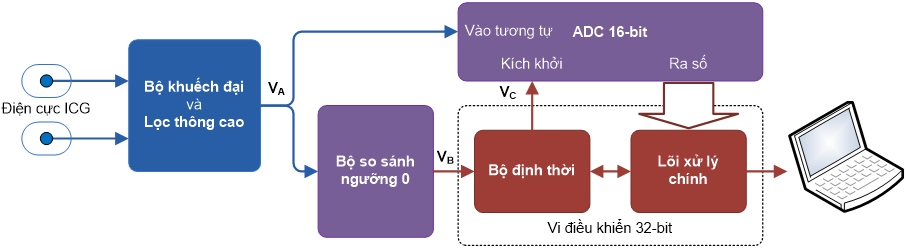
\includegraphics[height=4.39cm,width=16cm]{Images/Picture1.png}
    \caption[caption in table of content]{\bfseries Sơ đồ khối của hệ thống}
    \label{hinh21}
\end{figure}
\vspace{-18pt}
Hình \ref{hinh21} là ví dụ về cách chèn hình ảnh. Lưu ý chú thích của hình vẽ được đặt ngay dưới hình vẽ. Tất cả các hình vẽ phải được đề cập đến trong phần nội dung và phải được phân tích và bình luận giống như mình đang làm nhé :D.
\subsection{Cách tạo bảng}
\begin{table}[H]
\centering
\caption[Kết quả thí nghiệm]{\bfseries Kết quả thí nghiệm}
\label{bang21}
\begin{tabularx}{0.85\textwidth} { 
  | >{\centering\arraybackslash}s 
  | >{\centering\arraybackslash}X 
  | >{\centering\arraybackslash}a 
  | >{\centering\arraybackslash}s|}
 \hline
\bfseries Lần thí nghiệm & \bfseries Điện áp đo được\hspace{} (mV) &\bfseries  Điện áp tham chiếu \hspace{} (mV) & \bfseries Sai lệch\hspace{} (\%)\\
 \hline
1  &  &  & \\
 \hline
  2  &  &  & \\
 \hline
   3  &  &  & \\
 \hline
...  &  &  & \\
\hline
\end{tabularx}
\end{table}
Bảng \ref{bang21} là ví dụ về cách tạo bảng. Lưu ý chú thích của bảng được đặt trước bảng. Tất cả các bảng phải được đề cập đến trong phần nội dung và phải được phân tích và bình luận giống như mình đang làm nhé :D.
\subsection{Cách viết phương trình}
\begin{equation}\label{ptrinh1}
  F(x) &= \int^a_b \frac{1}{3}x^3 
\end{equation}
Phương trình (\ref{ptrinh1}) là ví dụ về phương trình tích phân.

Thử phương trình khác nhé.
\begin{equation} \label{ptrinh2}
x[t_n] = \frac{1}{\sqrt{N}} \sum_{k=0}^{N-1}X[f_k]e^{j 2 \pi n k/N},
\end{equation}
Phương trình (\ref{ptrinh2}) thể hiện phép biến đổi Fourier rời rạc ngược (IDFT).
\subsection{Cách viết định nghĩa, định lý, hệ quả, bổ đề}
Định lý lấy mẫu Nyquist–Shannon là một định lý được sử dụng trong lĩnh vực lý thuyết thông tin, đặc biệt là trong viễn thông và xử lý tín hiệu do Harry Nyquist và Claude Shannon phát minh.
\begin{theorem}\label{nyquist}
Một hàm số tín hiệu $x(t_n)$ không chứa bất kỳ thành phần tần số nào lớn hơn hoặc bằng một giá trị $f_m$ có thể biểu diễn chính xác bằng tập các giá trị của nó với chu kỳ lấy mẫu $ T = 1/(2f_m).$
\end{theorem}
Định lý \ref{nyquist} thường được gọi đơn giản là định lý lấy mẫu.
\begin{corollary}
There's no right rectangle whose sides measure 3cm, 4cm, and 6cm.
\end{corollary}
\begin{lemma}
Given two line segments whose lengths are $a$ and $b$ respectively there is a 
real number $r$ such that $b=ra$.
\end{lemma}
\begin{defn}
this is something about any defination...
\end{defn}
\newpage
\section*{\centering CHƯƠNG 4. THÍ NGHIỆM VÀ KẾT QUẢ}
\setcounter{section}{4}
\setcounter{subsection}{0}
\setcounter{figure}{0}
\setcounter{table}{0}
\phantomsection \addcontentsline{toc}{section}{\numberline{}CHƯƠNG 4. THÍ NGHIỆM VÀ KẾT QUẢ}
\lipsum
\newpage




%  conclusion
\section*{\centering KẾT LUẬN}
\phantomsection \addcontentsline{toc}{section}{\numberline{}KẾT LUẬN}
\subsection*{Kết luận chung}
\phantomsection \addcontentsline{toc}{section}{\numberline{}Kết luận chung}
Kết luận chung cho các chương trong đồ án. Mục này cần nhấn mạnh những vấn đề đã giải quyết và vấn đề chưa giải quyết để đưa ra các đánh giá về mức độ hoàn thành công việc. Đánh giá này thường bao gồm việc so sánh kết quả thu được với mục tiêu đề ra ban đầu.
\subsection*{Hướng phát triển}
\phantomsection \addcontentsline{toc}{section}{\numberline{}Hướng phát triển}
(Nếu có)
\subsection*{Kiến nghị và đề xuất}
\phantomsection \addcontentsline{toc}{section}{\numberline{}Kiến nghị và đề xuất}
(Nếu có)
\newpage
% Reference
\phantomsection \addcontentsline{toc}{section}{\numberline{}TÀI LIỆU THAM KHẢO}
\bibliographystyle{IEEEtran}
\bibliography{bibliography_twp}
\newpage
\section*{\centering PHỤ LỤC}
\phantomsection \addcontentsline{toc}{section}{\numberline{}PHỤ LỤC}
\texttt{\fontsize{10pt}{0pt}\selectfont Mã nguồn chương trình (nếu có) được đưa vào đây,  sử dụng font Courier New, cỡ 10
}
% \begin{table}[]
%     \centering
%     \begin{tabular}{0.85\textwidth}{|s|X[2]|d|d|d|d|d|}
%  \hline
%  \multicolumn{7}{Có sự kết hợp giữa lý thuyết và thực hành (20)} \\
%  \hline
% 1& Nêu rõ tính cấp thiết và quan trọng của đề tài, các vấn đề và các giả thuyết (bao gồm mục đích và tính phù hợp) cũng như phạm vi ứng dụng của đồ án & 1 & 2 & 3 & 4 & 5 & \\
%  \hline
%  2  & Cập nhật kết quả nghiên cứu gần đây nhất (trong nước/quốc tế) & 1 & 2 & 3 & 4 & 5 & \\
%   \hline
% 3&  Nêu rõ và chi tiết phương pháp nghiên cứu/giải quyết vấn đề  & 1 & 2 & 3 & 4 & 5 & \\
%  \hline
% 4 & Có kết quả mô phỏng/thực nghiệm và trình bày rõ ràng kết quả đạt được & 1 & 2 & 3 & 4 & 5 & \\
%  \hline
% \end{tabular}
%     \caption{Caption}
%     \label{tab:my_label}
% \end{table}
\end{document}
